\newpage
\section{Process Environment}


% Kill di un processo in C
\subsection{Kill di un processo in C}

Per far \hl{terminare un processo} usiamo:

\begin{enumerate}
    \item \hl{return} dal main
    \item chiamando \hl{exit}: \textbf{chiudo la singola thread} ma poi passa da un \textbf{gestore di exit (exit function)} che chiama gli \txtbf{exit handler} che possono essere installati e aggiunti tramite la funzione
\begin{lstlisting}
int atexit(void (*func)(void));
\end{lstlisting}
    e verranno richiamate in ordine contrario alla dichiarazione
    
    \item chiamando \hl{\_exit o \_Exit}: usate per terminare il processo e \textbf{finire direttamente nel kernel} senza passare dall'exit function
    \item \hl{return dell'ultima thread}
    \item chiando \hl{pthread\_exit dall'ultima thread}
    \item chiamando \hl{abort}: che \textbf{genera un segnale gestibile SIGABRT}, ma che fa comunque teminare il processo
    \item ricevendo un \hl{segnale}: come \textbf{SIGKILL e SIGSTOP} che non potranno essere gestiti o fermati
    \item \hl{richiesta di cancellazione} dell'ultima thread
\end{enumerate}


% Environment list
\subsection{Environment list}

Quando si va a \hl{creare una variabile} nello schell:

\begin{lstlisting}
$ a=100
\end{lstlisting}

questa \hl{non viene passara al child schell}, come "env", a meno di non \hl{usare il builtin "export"}.

In un processo \hl{possiamo vedere le variabli di ambiente in runtime}, tramite il debugger, ma non nello stesso punto in cui si trovano. \hl{Per le variabili di ambiente} abbiamo che:


\begin{figure}[H]
\centering
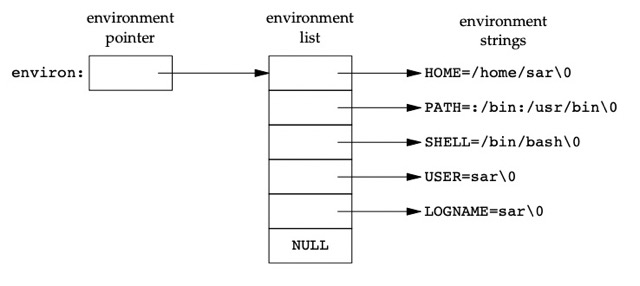
\includegraphics[scale=0.4]{varamb.jpeg}
\caption{Variabili di ambiente} 
\label{varamb}
\end{figure}


dove ogni valore è \hl{separato da un null $\backslash 0$} e \hl{storicizzato in un array di puntatori} andando a terminare con un null.

I programmi, tramite un \hl{handle}, possono \hl{accedere a questo array tramite un altro puntatore} (environment pointer), come:

\begin{lstlisting}
extern char **environ;
\end{lstlisting}

oppure nel \hl{main}:
\begin{lstlisting}
int main(int argc, char *argv[], char *envp[]);
\end{lstlisting}

oppure con la \hl{funzione}:
\begin{lstlisting}
char *getenv(const char *name);
\end{lstlisting}

che \hl{passando il nome della variaible di ambiente restituendo un puntatore al suo contenuto}.

Notare che la \hl{malloc usa zone globali allora non è rientrant}, vedremo poi cosa vuol dire.






(VEDERE memory\_dump.c) che vede e sampa tutte le variabili di mabinete, aspetta un p`o e poi lo ri fa stampandone anche di nuove e modificandone una esistente e poi va a vedere rispetto ai punttori precendenti c se sno ancora buoni  o se stanno da un altra parte 

vedere a mush simpler way to print addresses used in process memory per stampare semplicemtne gli indirizzi delle variabili di ambiente